% -*- mode: latex; mode: reftex; mode: outline-minor -*-
\documentclass{jsarticle}
\usepackage{amsmath,amssymb}
\usepackage[dvipdfmx]{graphicx}
\usepackage{booktabs}
\usepackage{url}
\usepackage[framemethod=tikz]{mdframed}

\title{mhwスキルシミュレータと線形計画法
\\
{\small 4版. 2021年1月11日}
}
\date{}
\author{5chスキルシミュレータ開発Ver.13の480}

\begin{document}
\maketitle
\tableofcontents

\section{線形計画法}
{\bf 線形計画問題}とは、1次方程式や不等式で条件が与えられた変数たちがあるとき、
目的の1次式を最大、あるいは、最小にするような変数たちの値を解として求める問題を言い、
その解法を{\bf 線形計画法}と呼びます。

例えば、次の条件 (あ)
%
\begin{align*}
x \geqq 0 , \qquad
y \geqq 0 , \qquad
\dfrac{x}{6} + \dfrac{y}{8} \leqq 1 , \qquad
\dfrac{x}{10} + \dfrac{y}{3} \leqq 1
\tag{あ}
\end{align*}
%
を満たすように変数$x$, $y$が動くとき、1次式
\begin{align*}
k = x + 2y
\end{align*}
の最大値と、そのときの$x$, $y$の値を求めよというような問題です。

筆者が昔、高校で習った解法は次の通りです。
条件 (あ) を満たす$(x,y)$の領域を平面に図示すると、
下図左の四角形OAPDの内部と周になります。
$k = x+2y$は、
$y = -\frac{1}{2}x + \frac{k}{2}$と変形して、
傾き$-1/2$、$y$切片$k/2$の直線の方程式だと思います。
これを、四角形OAPDを通過するように、なおかつ、
切片$k/2$ が最大 (つまり$k$も最大) になるようにかくと、
点P$(\frac{150}{31}, \frac{48}{31})$を通過するような、
下図左に赤く記した直線になります。
従って、$k$の最大値は、
$k = x + 2y = \frac{246}{31}$と求まります。

\bigskip
\noindent
\hfil
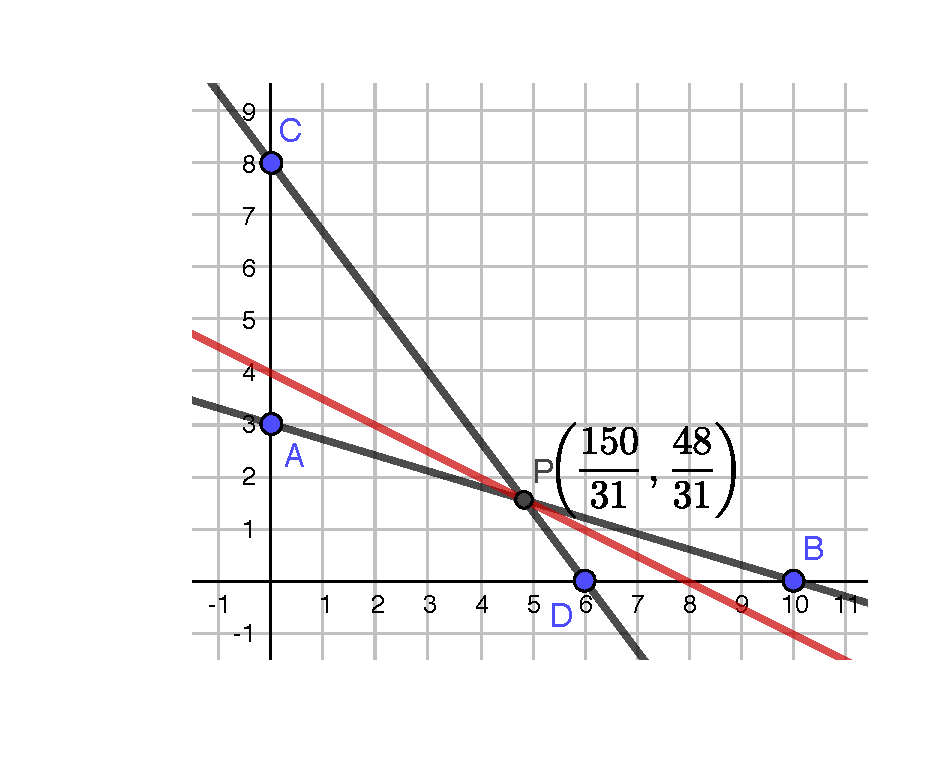
\includegraphics[scale=0.65]{./fig/lpgraph2.pdf}
\hfil
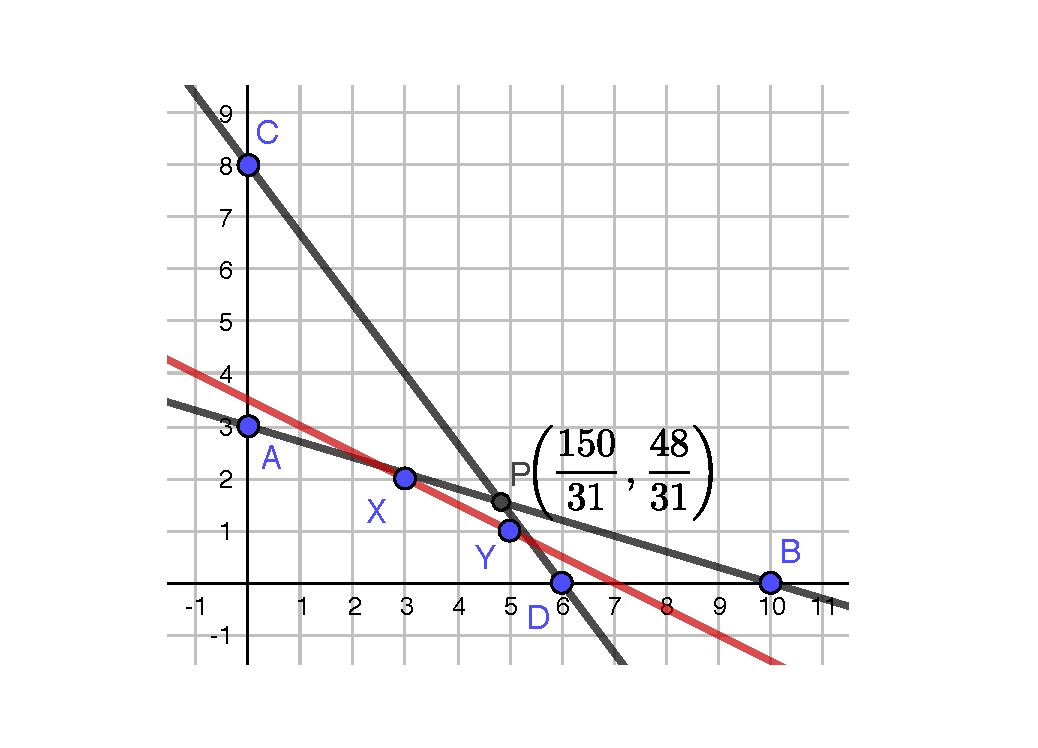
\includegraphics[scale=0.65]{./fig/lpgraph3.pdf}
\hfil
\bigskip

また、変数$x$, $y$を整数に限定すると、
同様に考えたときに、点Pを通過するのでは$x$, $y$が整数にならないので、
四角形OAPDの内部または周上の格子点 (座標成分が整数になる点) を通るように、
なおかつ、切片$k/2$が最大になるように、傾き$-1/2$の直線をかくと、
上図右の直線XYになります。
つまり、整数解は、$(x,y) = (3,2), (5,1)$の2通りで、
$k = x+2y = 7$が最大値です。

このように線形計画問題であって、整数解を求める問題を{\bf 整数計画問題}と呼びます。
%
線形計画問題や整数計画問題は、非常に応用範囲の広い問題なので、
計算機で高速に解く方法が研究され多くの実装が公開されています。

mhwのスキルシミュレータの高速なアルゴリズムを考える時に、
例えばLv4の装飾品を特別に扱うとか、シリーズスキルを特別に扱うとか、
問題固有の工夫で高速化を追求することが多いように思いますが、
こういった問題固有の工夫を考える場合、どの工夫が有効か無効かを実際に試して、
有効なものを実装する、という手間が必要で、
工夫を盛り込めば盛り込む程、プログラムも複雑化・肥大化します。
%
しかし、整数計画問題に帰着させれば、これらの手間をかけずに、
既存の高速な整数計画問題ライブラリが勝手に高速化してくれ
(ると、期待でき) ます。
少なくとも、プログラムを書く手間は劇的に減ります。
%
筆者は、2019年9月21日の時点ではまともなGUIがないので公開はしていませんでした。
9月23日には、5chスキルシミュレータ開発Ver.13の496さんがGUIをつけて下さり、
その後、線形計画法の部分も独自に書き直して、
線形計画法を用いてスキルシミュレータを公開されています
(\url{https://imasanari.github.io/mhw-simulator/})。
筆者も、
2019年10月18日現在、暫定的なものを公開しています
(\url{http://nap.s3.xrea.com/lpsim.html})。

本原稿の目的は、
スキルシミュレータのアルゴリズムを整数計画問題に帰着させる方法の解説です。
この方法を活用して素晴しいスキルシミュレータを作る方が
たくさん現れたら良いなと思います。

\section{整数計画問題への帰着}
\subsection{防具・護石・装飾品・スキルの数}
あまり実害はないと思いますが、
「ゲラルト$\alpha$」のようなワンセット防具は、当面の間考えないことにします。
武器スロットや汎用スロットも当面は考えないことにします。
\ref{subsec:kuwashii-kensaku}に後述します。

ワンセット防具を除いた防具、護石、装飾品の種類の数、
また、シリーズスキルも含めたスキルの種類の数は、次の表の通りとします。
\begin{quote}
\begin{tabular}{lccccccc}
\toprule
{}        & 頭防具 & 胴防具 & 腕防具 & 腰防具 & 脚防具 & 護石 & 装飾品 \\
種類の数  & $e_1$ & $e_2$ & $e_3$ & $e_4$ & $e_5$ &  $c$ & $d$  
\\ \bottomrule
\end{tabular}
\quad (ワンセット防具除く)
\bigskip
\\
\begin{tabular}{lccccccc}
\toprule
{}        & スキル\\
種類の数  & $n$
\\ \bottomrule
\end{tabular}
\quad (シリーズスキル含む)
\end{quote}
%
$e_1, \ldots, e_5$や$c, d$はだいたい200から400くらいの値で、
$n$も400くらいです。

\subsection{係数ベクトル}

各防具・護石・装飾品に対し、次のベクトルを定めます。
これを{\bf 係数ベクトル}と呼ぶことにします。
係数ベクトルは$(n+11)$次の、整数を成分に持つ縦ベクトルで、その成分は次の通りです。
\begin{center}
\begin{tabular}{llllllllllllllll}
\toprule
成分 & 意味 & 説明 \\
\midrule
1 & 頭防具カウンタ & 頭防具なら1。その他の防具、護石、装飾品なら0 \\
2 & 胴防具カウンタ &  胴防具なら1。その他の防具、護石、装飾品なら0 \\
3 & 腕防具カウンタ &  腕防具なら1。その他の防具、護石、装飾品なら0 \\
4 & 腰防具カウンタ &  腰防具なら1。その他の防具、護石、装飾品なら0 \\
5 & 脚防具カウンタ &  脚防具なら1。その他の防具、護石、装飾品なら0 \\
\midrule
6 & 護石カウンタ   &  護石なら1。防具、装飾品なら0 \\
\midrule
7 & Lv1以上スロット & 防具のLv1以上のスロット数。装飾品なら負にする。\\
8 & Lv2以上スロット & 防具のLv2以上のスロット数。装飾品なら負にする。\\
9 & Lv3以上スロット & 防具のLv3以上のスロット数。装飾品なら負にする。\\
10 & Lv4以上スロット & 防具のLv4以上のスロット数。装飾品なら負にする。\\
\midrule
11 & 防御力 & 防具の防御力。護石・装飾品なら0 \\
\midrule
12--($n+11$) & スキル & スキルがあれば、そのスキルポイント。
\\ \bottomrule
\end{tabular}
\end{center}

スロットの部分とスキルの部分について補足をします。
まず、スキルですが、
$n$種類のスキルには
スキル1は攻撃、スキル2は渾身、スキル3は見切り、$\cdots$、スキル$n$は滅尽龍の覇気、
のように適当に番号を付けておきます。
例えば、防具に攻撃Lv1と見切りLv2が付いているなら、
係数ベクトルのスキルの部分、つまり、係数ベクトルの第12成分以降は、
$(1, 0, 2, \ldots, 0)$とします。
%
装飾品の場合も同様です。

次にスロットの部分ですが、
防具にスロットがいくつか付いているとき、
いくつかの装飾品が装着できるかどうかは、
\begin{align*}
(\text{防具のLv1スロット数}) \geqq (\text{Lv1スロットを必要とする装飾品数}) \\
(\text{防具のLv2スロット数}) \geqq (\text{Lv2スロットを必要とする装飾品数}) \\
(\text{防具のLv3スロット数}) \geqq (\text{Lv3スロットを必要とする装飾品数}) \\
(\text{防具のLv4スロット数}) \geqq (\text{Lv4スロットを必要とする装飾品数}) 
\end{align*}
と判定してはいけないです。
なぜなら、Lv2スロットにもLv1装飾品は装着できるからです。

Lv4装飾品はLv4スロットにしか装着できないので、上の4つ目の不等式はそのままでよいです。
Lv3装飾品はLv3かLv4のスロットに装着できるので、
$(\text{防具のLv3以上のスロット数}) \geqq (\text{Lv3スロットを必要とする装飾品数})$
としたいところですが、Lv4スロットはLv4装飾品でも消費されるので、
正しくは、
$(\text{防具のLv3以上のスロット数}) \geqq (\text{Lv3以上のスロットを必要とする装飾品数})$
です。
従って、まとめると、
\begin{align*}
(\text{防具のLv1以上のスロット数}) \geqq (\text{Lv1以上のスロットを必要とする装飾品数}) \\
(\text{防具のLv2以上のスロット数}) \geqq (\text{Lv2以上のスロットを必要とする装飾品数}) \\
(\text{防具のLv3以上のスロット数}) \geqq (\text{Lv3以上のスロットを必要とする装飾品数}) \\
(\text{防具のLv4以上のスロット数}) \geqq (\text{Lv4以上のスロットを必要とする装飾品数}) 
\end{align*}
が、
装着できるかどうかの条件になります。
%
これが係数ベクトルの第7--10成分が、Lv1「以上」のスロット数、などとなっている理由です。

例えば、
Lv2スロット1つと
Lv4スロット1つが付いている防具だと、
係数ベクトルの第7--10成分は、$(2,2,1,1)$となります。
%
また、Lv3スロットを必要とする装飾品では、$(-1,-1,-1,0)$となります。
防具を装備すればスロットが増加しますが、
装飾品の場合は装備すればスロットを消費するので負にします。

\subsection{係数ベクトルの例}
\paragraph{頭防具: エンプレスセクター$\alpha$}
Lv3スロット1つ、
Lv1スロット1つ、
回避距離UPのスキルポイントが2、
整備のスキルポイントが1
ついていて、
カスタム強化後の防御力は90です。
%
この係数ベクトルは、転置して横ベクトルで書くと、
\begin{align*}
(
\underbrace{1,0,0,0,0}_{\text{防具カウンタ}},
\underbrace{0}_{\text{護石カウンタ}},
\underbrace{2,1,1,0}_{\text{スロット}},
\underbrace{90}_{\text{防御力}},
\underbrace{0,\ldots, 2, \ldots, 1, \ldots ,0}_{\text{スキル}}
)
\end{align*}
となります。
スキルの部分は、
回避距離UPに対応する成分に2、
整備に対応する成分に1となります。

\paragraph{護石: 堅守の護石}
ガード強化のスキルポイントが1、
死中に活のスキルポイントが1ついています。
%
この係数ベクトルは、転置して横ベクトルで書くと、
\begin{align*}
(
\underbrace{0,0,0,0,0}_{\text{防具カウンタ}},
\underbrace{1}_{\text{護石カウンタ}},
\underbrace{0,0,0,0}_{\text{スロット}},
\underbrace{0}_{\text{防御力}},
\underbrace{0,\ldots, 1, \ldots, 1, \ldots ,0}_{\text{スキル}}
)
\end{align*}
となります。
スキルの部分は、
ガード強化と死中に活に対応する成分が1です。

\paragraph{護石: 威嚇の護石III}
威嚇のスキルポイントが3ついています。
%
この係数ベクトルは、転置して横ベクトルで書くと、
\begin{align*}
(
\underbrace{0,0,0,0,0}_{\text{防具カウンタ}},
\underbrace{1}_{\text{護石カウンタ}},
\underbrace{0,0,0,0}_{\text{スロット}},
\underbrace{0}_{\text{防御力}},
\underbrace{0,\ldots, 3, \ldots ,0}_{\text{スキル}}
)
\end{align*}
となります。
スキルの部分は、威嚇に対応する成分が3です。

\paragraph{装飾品: 回避珠【2】}
必要スロットはLv2で、
回避性能のスキルポイントが1ついています。
%
この係数ベクトルは、転置して横ベクトルで書くと、
\begin{align*}
(
\underbrace{0,0,0,0,0}_{\text{防具カウンタ}},
\underbrace{0}_{\text{護石カウンタ}},
\underbrace{-1,-1,0,0}_{\text{スロット}},
\underbrace{0}_{\text{防御力}},
\underbrace{0,\ldots, 1, \ldots ,0}_{\text{スキル}}
)
\end{align*}
となります。
スキルの部分は、回避性能に対応する成分が1です。

\paragraph{装飾品: 滑走・攻撃珠【4】}
必要スロットはLv4で、
滑走のスキルポイントが1、
攻撃のスキルポイントが1ついています。
%
この係数ベクトルは、転置して横ベクトルで書くと、
\begin{align*}
(
\underbrace{0,0,0,0,0}_{\text{防具カウンタ}},
\underbrace{0}_{\text{護石カウンタ}},
\underbrace{-1,-1,-1,-1}_{\text{スロット}},
\underbrace{0}_{\text{防御力}},
\underbrace{0,\ldots, 1, \ldots, 1, \ldots ,0}_{\text{スキル}}
)
\end{align*}
となります。
スキルの部分は、滑走と攻撃に対応する成分が1です。

\subsection{整数計画問題}

防具、護石、装飾品の総数は$e_1+e_2+e_3+e_4+e_5+c+d$ですが、
この個数の変数
$x_1, x_2, \ldots, x_{e_1+e_2+e_3+e_4+e_5+c+d}$
を考えます。
これらは、スキルシミュレータで出力される装備で、
どの防具・護石・装飾品を何個使っているかを意味する、
0以上の整数の値をとる変数です。
%
\begin{align*}
x_i \geqq 0 \quad (i = 1,2,\ldots, e_1+e_2+e_3+e_4+e_5+c+d)
\tag{条件1}
\end{align*}

次に、$(n+11) \times (e_1+e_2+e_3+e_4+e_5+c+d)$行列$M$
(だいたい$200 \times 2000$) を、
各列に防具・護石・装飾品の係数ベクトルを並べることで作ります。
係数ベクトルを並べる順番は、
頭防具 ($e_1$列あります)、
胴防具 ($e_2$列あります)、
腕防具 ($e_3$列あります)、
腰防具 ($e_4$列あります)、
脚防具 ($e_5$列あります)、
護石   ($c$列あります)、
装飾品 ($d$列あります) の順です。

そして、これらの間の関係式
\begin{align*}
\begin{pmatrix}
y_1 \\ y_2 \\ \vdots \\ y_{n+11}
\end{pmatrix}
=
M
\begin{pmatrix}
x_1 \\ x_2 \\ \vdots \\ x_{e_1+e_2+e_3+e_4+e_5+c+d}
\end{pmatrix}
\tag{$y$と$x$の関係式}
\end{align*}
を考えます。
%
すると、
$y_i$は、各防具・護石・装飾品の係数ベクトルの第$i$成分の1次結合です。
つまり、
\begin{align*}
y_i &= 
(\text{1番目の防具の係数ベクトルの第$i$成分}) x_1 +
\\ &\quad\quad
(\text{2番目の防具の係数ベクトルの第$i$成分}) x_2 +
\cdots +
\\ &\quad\quad
(\text{最後の装飾品の係数ベクトルの第$i$成分}) x_{e_1+e_2+e_3+e_4+e_5+c+d}
\end{align*}
です。
%
従って、
$x_1, x_2, \ldots, x_{e_1+e_2+e_3+e_4+e_5+c+d}$で決まる装備に対して、
$(n+11)$個の変数$y_1, y_2, \ldots, y_{n+11}$は次のような意味を持ちます。
%
\begin{center}
\begin{tabular}{llllllllllllllll}
\toprule
$y_i$ & 意味 \\
\midrule
$y_1$ & 頭防具の個数 \\
$y_2$ & 胴防具の個数 \\
$y_3$ & 腕防具の個数 \\
$y_4$ & 腰防具の個数 \\
$y_5$ & 脚防具の個数 \\
\midrule
$y_6$ & 護石の個数 \\
\midrule
$y_7$ & (防具のLv1以上スロット数)$-$(Lv1以上のスロットを必要とする装飾品数) \\
$y_8$ & (防具のLv2以上スロット数)$-$(Lv2以上のスロットを必要とする装飾品数) \\
$y_9$ & (防具のLv3以上スロット数)$-$(Lv3以上のスロットを必要とする装飾品数) \\
$y_{10}$&(防具のLv4以上スロット数)$-$(Lv4以上のスロットを必要とする装飾品数) \\
\midrule
$y_{11}$ & 防具5部位の合計防御力 \\
\midrule
$y_{12}$--$y_{n+11}$ & スキルごとの発動スキルポイント
\\ \bottomrule
\end{tabular}
\end{center}
%
従って、$y_i$は次の条件を満たす必要があります。
%
\begin{align*}
& 0 \leqq y_i \leqq 1 \quad (i = 1,2,3,4,5,6) \quad  \text{(防具・護石は部位ごとに1つまで)}
\tag{条件2}
\\
& 0 \leqq y_i \hspace{10mm} (i = 7,8,9,10)  
\hspace{8.3mm} \text{(スロットが足りているなら差し引き0以上のはず)}
\tag{条件3}
\end{align*}

スキルシミュレータでは、どれだけのスキルを発動させたいかを自分で設定して検索をかけますが、
スキル1からスキル$n$までの発動させたいスキルポイントを、順に、
$s_1, s_2, \ldots, s_n$ とすると、
$y_{12}$からがスキルの変数なので、番号付けのズレも考慮すると、
次の条件が必要です。
%
\begin{align*}
y_{11+i} \geqq s_i \quad (i = 1,2,\ldots, n)
\tag{条件4}
\end{align*}

最後に、線形計画法では、何かを最大化するのですが、
防御力を最大化するなら、
\begin{align*}
y_{11} \text{を最大化する}
\tag{最大化a}
\end{align*}
となります。
他の意味のありそうな最大化としては、
Lv1以上の空きスロット数、つまり、全空きスロット数を最大化したいならば、
\begin{align*}
y_{7} \text{を最大化する}
\tag{最大化b}
\end{align*}
とすればよいです。
Lv2以上やLv3以上の空きスロット数を最大化したい場合の話は後述します。
また、
$s_i$で指定したスキルポイントに加えて、
あるスキルを付けられるだけ付けたいならば、
そのスキルポイントを最大化すればよいので、
例えばスキル1ならば、最大スキルポイントを7すると、
\begin{align*}
y_{12} \leqq 7, \quad
y_{12} \text{を最大化する}
\tag{最大化c}
\end{align*}
とすればよいです。
ただし、細かいことですが、防具だけでスキルポイントの上限
を超える場合、それが検索対象であるにも関わらず、
検索から漏れてしまうので注意が必要です。

以上をまとめると、
スキルシミュレータのアルゴリズムを整数計画問題に帰着させるには、
次のようにすればよいことがわかりました。
%
\begin{mdframed}
\hfil
\begin{minipage}{0.8\textwidth}
{\bf 変数} $x_i$ ($i=1,2,\ldots,e_1+e_2+e_3+e_4+e_5+c+d$) \\
{\bf 変数} $y_i$ ($i=1,2,\ldots,n$) \\
に対し、制約条件\\
{\bf ($y$と$x$の関係式)}
$\overrightarrow{y} = M \overrightarrow{x}$
\\
{\bf (条件1)}
$x_i \geqq 0 \hspace{9.8mm} (i = 1,2,\ldots, e_1+e_2+e_3+e_4+e_5+c+d)$
\\
{\bf (条件2)}
$ 0 \leqq y_i \leqq 1 \quad (i = 1,2,3,4,5,6)$
\\
{\bf (条件3)}
$ 0 \leqq y_i \hspace{10mm} (i = 7,8,9,10)  $
\\
{\bf (条件4)}
 $y_{11+i} \geqq s_i \hspace{4mm} (i = 1,2,\ldots, n)$
\\
の下で、\\
{\bf (最大化a)}
 $y_{11}$ を最大化する
\\
ことを行い、
解があれば、$x_i$のうち0ではないものが求める装備の個数であり、
防御力が最大のものが求まっている。
\end{minipage}
\end{mdframed}

\subsection{より詳しい検索} \label{subsec:kuwashii-kensaku}
\paragraph{防具・護石の除外、装飾品の個数制限}
例えば、頭防具の1番目を除外したいならば、その個数が$x_1$ですから、
\begin{align*}
x_1 = 0 
\tag{防具の除外}
\end{align*}
という制約条件を追加すればよいですし、
護石の1番目を除外したいならば、その個数は
$x_{e_1+e_2+e_3+e_4+e_5+1}$ですから、
\begin{align*}
x_{e_1+e_2+e_3+e_4+e_5+1} = 0 
\tag{護石の除外}
\end{align*}
という制約条件を追加すればよいです。

また、装飾品の1番目の個数を4個以下に制限して検索をしたいならば、
\begin{align*}
x_{e_1+e_2+e_3+e_4+e_5+c+1} \leqq 4
\tag{装飾品の個数制限}
\end{align*}
という制約条件を追加すればよいです。

\paragraph{武器スロット・汎用スロット}
武器にスロットが付いていれば、(条件3)が変更されます。
防具や装飾品のスロットの場合と同様に、武器に対しても、
\begin{align*}
t_7    &= (\text{武器のLv1以上のスロット数}) \\
t_8    &= (\text{武器のLv2以上のスロット数}) \\
t_9    &= (\text{武器のLv3以上のスロット数}) \\
t_{10} &= (\text{武器のLv4以上のスロット数})
\end{align*}
と定め、
(条件3) $0 \leqq y_i$ の代わりに、
$0 \leqq y_i + t_i$ とすればよいです。

さらに、汎用スロットを確保したいということであれば、
使用できるスロットが減るわけですから、
\begin{align*}
u_7    &= (\text{Lv1以上の汎用スロット数}) \\
u_8    &= (\text{Lv2以上の汎用スロット数}) \\
u_9    &= (\text{Lv3以上の汎用スロット数}) \\
u_{10} &= (\text{Lv4以上の汎用スロット数})
\end{align*}
と定め、
(条件3) $0 \leqq y_i$ の代わりに、
$0 \leqq y_i + t_i - u_i$ とすればよいです。

まとめると、(条件3)の代わりに、
\begin{align*}
0 \leqq y_i + t_i - u_i
\quad (i = 7,8,9,10)  
\qquad \text{(スロットが足りているなら差し引き0以上のはず)}
\tag{条件3$'$}
\end{align*}
を用いるとよいことになります。

\paragraph{ワンセット防具}
ここまでの解説では「ゲラルト$\alpha$」のような
ワンセット防具は除外して考えましたが、
これも含めて検索を行う方法を説明します。

ワンセット防具を含めた場合も、係数ベクトルの作り方や、
(条件1)から(条件4)などの制約条件は同じです。

そして、例えば、ワンセット防具「ゲラルト$\alpha$」の
頭、胴、腕、腰、脚が順に、
$x_{g_1}$, $x_{g_2}$, $x_{g_3}$, $x_{g_4}$, $x_{g_5}$
で個数を表しているとすると、
これらはすべて使うか、すべて使わないかの
いずれかですから、以下のような条件が追加されます。
%
\begin{align*}
x_{g_1} = x_{g_2} = x_{g_3} = x_{g_4} = x_{g_5}
\tag{ワンセット防具の条件}
\end{align*}
%
他のワンセット防具についても、同様の条件を追加すればよいです。

\paragraph{得られた解における空きスロット数}
整数計画問題の解が得られたとき、
空きスロットがいくつあるかは、次のようにするとわかります。
例えば、Lv2以上のスロットが$a$個以上空いているということは、
何かLv2の装飾品を$a$個追加で付けても、
(条件3) が成立するということなので、
\begin{align*}
&\text{(防具のLv1以上スロット数)}-
\text{(Lv1以上のスロットを必要とする装飾品数)} -a \geqq 0 \\
&\text{(防具のLv2以上スロット数)}-
\text{(Lv2以上のスロットを必要とする装飾品数)} -a \geqq 0 \\
&\text{(防具のLv3以上スロット数)}-
\text{(Lv3以上のスロットを必要とする装飾品数)} \geqq 0 \\
&\text{(防具のLv4以上スロット数)}-
\text{(Lv4以上のスロットを必要とする装飾品数)} \geqq 0 
\end{align*}
つまり、
\begin{align*}
y_7 \geqq a, \quad
y_8 \geqq a, \quad
y_9 \geqq 0, \quad
y_{10} \geqq 0
\end{align*}
と表せます。
最大何個付けられるかがLv2以上の空きスロット数ですが、
$a$は最大$\min\{y_7, y_8\}$ ($y_7$と$y_8$の最小値) まで大きくできますから、
Lv2以上の空きスロット数は$\min\{y_7, y_8\}$です。

同様に考えて、整数計画問題の解が得られたときの、空きスロット数は、
\begin{center}
\begin{tabular}{llllllll}
\toprule
空きスロット & (条件3)のとき & (条件3$'$)のとき \\
\midrule
Lv1以上 & $\min\{y_7\}$
& $\min\{y_7+t_7-u_7\}$ \\
Lv2以上 & $\min\{y_7,y_8\}$ 
& $\min\{y_7+t_7-u_7,y_8+t_8-u_8\}$ \\
Lv3以上 & $\min\{y_7,y_8,y_9\}$ 
& $\min\{y_7+t_7-u_7,y_8+t_8-u_8,y_9+t_9-u_9\}$ \\
Lv4以上 & $\min\{y_7,y_8,y_9,y_{10}\}$
& $\min\{y_7+t_7-u_7,y_8+t_8-u_8,y_9+t_9-u_9,y_{10}+t_{10}-u_{10}\}$
 \\
\bottomrule
\end{tabular}
\end{center}
となります。
従って、
\begin{center}
\begin{tabular}{llllllll}
\toprule
空きスロット & (条件3)のとき \\
\midrule
Lv1 & $\min\{y_7\} - \min\{y_7,y_8\}$ \\
Lv2 & $\min\{y_7,y_8\} -\min\{y_7,y_8,y_9\}$  \\
Lv3 & $\min\{y_7,y_8,y_9\} - \min\{y_7,y_8,y_9,y_{10}\}$ \\
Lv4 & $\min\{y_7,y_8,y_9,y_{10}\}$
\\
\bottomrule
\end{tabular}
\end{center}
です。
(条件3$'$)の場合も同様ですが、長いので省略します。

\paragraph{スロット数の最大化}
Lv1以上の空きスロット数を最大化して整数計画問題を解く方法は、
既に説明しましたが、ここでは、
有用性は劣ると思われますが、Lv2以上やLv3以上の場合について説明します。
Lv2の空きスロットではなく、Lv2「以上」の空きスロット数を最大化する理由は、
Lv2のスロットが欲しいわけではなく、
Lv2のスロットを必要とする装飾品を装着したいからです。

前の項で述べたように、
Lv2以上の空きスロット数は、
$\min\{y_7,y_8\}$ですから、これを最大化すればよいです。
ただし、1次式で表さなくてはならないので、
このままでは整数計画問題に落とせません。

そこで、新しい変数$z_8$を用意して、
$y_7 \geqq z_8$,
$y_8 \geqq z_8$
と条件を置いて、$z_8$を最大化すればよいです。
同様に考えて、Lv1以上、Lv2以上、Lv3以上、Lv4以上
の空きスロット数を最大化するには、それぞれ、
%
\begin{align*}
& y_7 \text{を最大化する} \tag{Lv1空きスロット数を最大化}
\\
& y_7 \geqq z_8, \;  y_8 \geqq z_8, \; 
z_8 \text{を最大化する} \tag{Lv2空きスロット数を最大化}
\\
& y_7 \geqq z_9, \;  y_8 \geqq z_9, \; y_9 \geqq z_9,
z_9 \text{を最大化する} \tag{Lv3空きスロット数を最大化}
\\
& y_7 \geqq z_{10}, \;  y_8 \geqq z_{10}, \; y_{10} \geqq z_{10}, \; y_{10} \geqq z_{10},
z_{10} \text{を最大化する} \tag{Lv4空きスロット数を最大化}
\end{align*}
とすればよいです。

\paragraph{極意スキルによる上限解放}
mhwはアイスボーンから、「極意」スキルが登場しています。
通常「整備」は最大Lv3までですが、
「整備・極意」にあたる「炎妃龍の真髄」のLv3以上があれば、
「整備」がLv5まで上限解放されるといったものです。
可能な組合せは下図左で丸印を付けた格子点になります。

線形計画法では、1次不等式で領域を決めますので、
下図左のような凸ではない領域を指定することはできません。
しかし、整数計画問題ならば、変数が整数であることを利用して、
1次不等式のみでこの領域を指定することができます。
%
まず、「炎妃龍の極意」のスキルポイントを3で割り、切り捨てて整数にします。
すると、下図右の赤い直線上を含む直線の上側が可能な格子点の領域となり、
1次不等式で指定することができます。

\bigskip
\noindent
\hfil
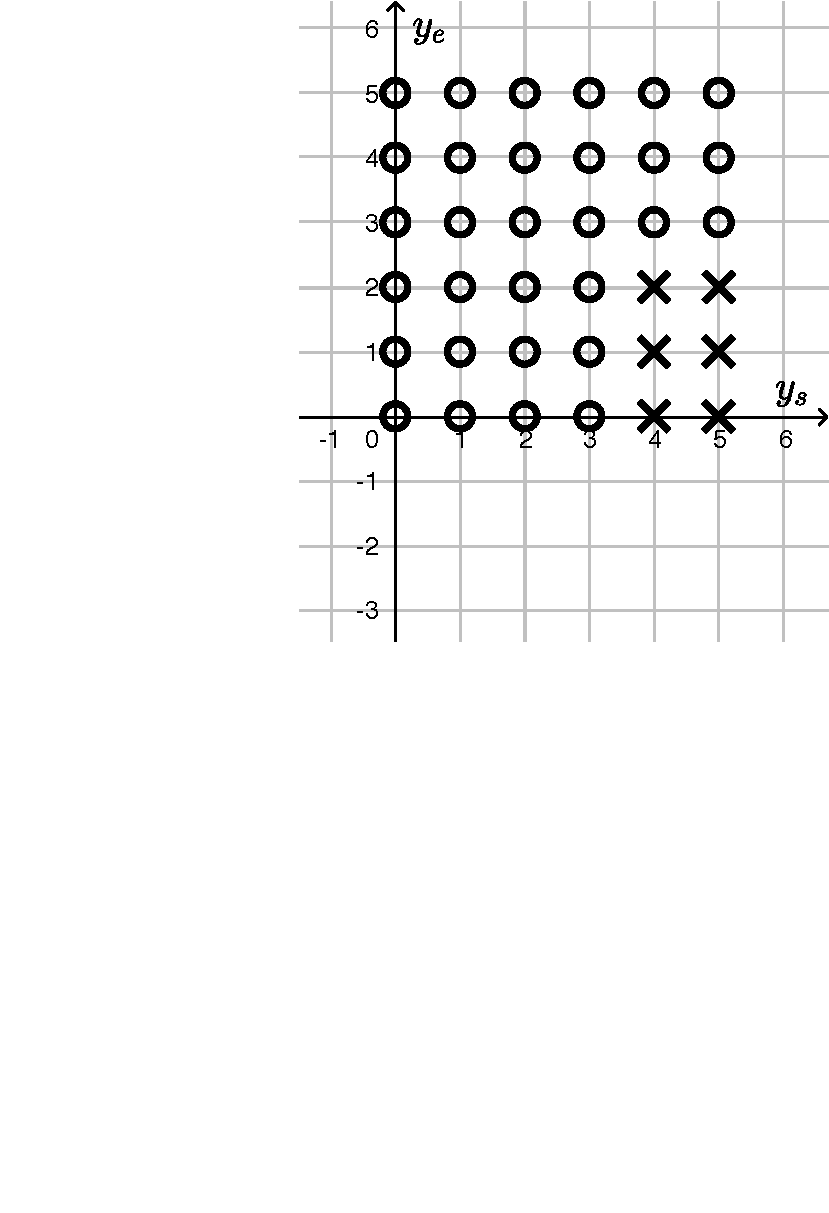
\includegraphics[scale=0.5]{./fig/lpgraph4.pdf}
\hfil
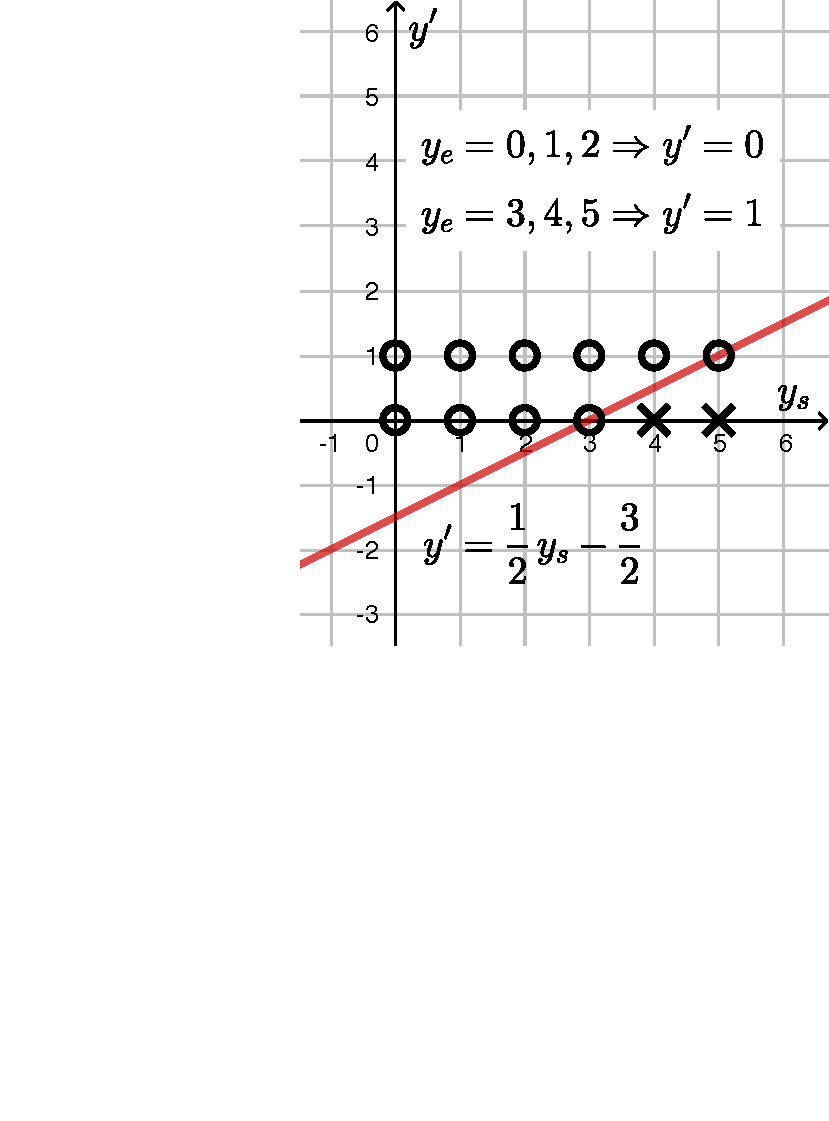
\includegraphics[scale=0.5]{./fig/lpgraph5.pdf}
\hfil
\bigskip

「整備」のスキルポイントを$y_s$、
「炎妃龍の真髄」のスキルポイントを$y_e$とし、
$y_e$を3で割り切り捨てた整数を表す
補助的な変数$y'$も用いると、
「炎妃龍の真髄」がLv3以上の場合のみ、「整備」がLv4以上になれるという条件は、
%
\begin{align*}
& 3 y' \leqq y_e \\
& 2 y' \geqq  - y_s -3
\end{align*}
と表せます。

この式は、「整備」など、極意がLv3で上限がLv3からLv5に解放される場合の式です。
「力の解放」や「満足感」のように、レベルの値が異なるときは別の式になりますが、
考え方は同じです。

\section{既知の問題点} \label{sec:known-bugs}
\paragraph{すべての組合せが検索されない}
整数計画問題をプログラムに解かせると、
解は1つだけ求まってプログラムは停止し、
すべてを見付けてはくれないのが普通だと思います。
つまり、条件に合う装備をすべて検索してくれるわけではありません。

スマートではありませんが、
次のようにすると、すべての装備を検索することはできます。

解が1つ見付かったとき、
その防具の頭、胴、腕、腰、脚、護石が順に、
$x_{h_1}$, $x_{h_2}$, $x_{h_3}$, $x_{h_4}$, $x_{h_5}$, $x_{h_6}$
で個数を表していたとします。
このとき、
\begin{align*}
x_{h_1} + x_{h_2} + x_{h_3} + x_{h_4} + x_{h_5} + x_{h_6}\leqq 5
\tag{検索済みの防具・護石の組合せを除外}
\end{align*}
という条件を追加して再び整数計画問題を解くと、
前回見付かった防具5部位と護石の組合せは除外されて別の検索結果が得られます。
%
これを、何度も反復すると、次々に異なる防具・護石・装飾品の組合せが得られます。

この方法では、検索結果1つにつき整数計画問題を1回実行するので、
既に公開されているスキルシミュレータよりは、かなり効率が悪くなると思います。
%
このようにするよりは、最初の検索結果の、
空きスロット数やおまけでついてきたスキル数を見て、
付けたいスキルを少し増やして再検索する方が、
実用的で意味のある方法だと思います。

(この段落は4版で追加)
整数計画問題をプログラムに解かせたとき、
プログラム停止時に解は1つだけ返りますが、
その過程では、多くの最良ではない解を発見していることが普通です。
つまり、条件に合う装備は、防御力最大ではないものも含めて、
複数発見していることが普通です。
%
線型計画法のライブラリに手を加えることで、
それらを取り出すことも可能なので、後述します。

\paragraph{実行速度}
Javascriptだと整数計画問題を解くのが遅いとか、
高速化の工夫をしていないから遅いということは、もちろんあります。
それとは質の違う課題として、変数の数や不等式の数が少なくても、
問題によっては非常に時間がかかるという、
整数計画問題独特の課題があります。
例えば、攻撃Lv7、防御Lv7、体力増強Lv3だとすぐに見付かるけれど、
体力増強をLv2にすると非常に時間がかかる、
といったような、コントロールのできない状況が発生します。

対策の1つとしては、時間がかかりそうだったら、スキルの条件を1つ追加するなどして、
条件を少し変えて検索をすることがあります。
ただ、こうすれば早くなるという万能な対策は恐らくないと思われます。

\section{実装上の補足}
\paragraph{線形計画法のライブラリ}
線形計画法のライブラリについては、筆者はあまり詳しくありませんが、
既存のライブラリを使うのが筋でしょう。
自作した場合は性能を出すための苦労が増えますし、
その苦労をしないために、整数計画問題に帰着させたわけですから。

無償で利用できるライブラリとしては、以下のようなものがあります、
と表にするつもりでしたが、調べるのが面倒なので3つだけです。
%
\begin{center}
\begin{tabular}{lllll}
\toprule
ライブラリ & & 言語 \\
\midrule
GLPK & (GNU Linear Programming Kit) & C \\
& \url{https://www.gnu.org/software/glpk/}
\\
glpk.js & (JavaScript port of GLPK) & JavaScript \\
& \url{https://github.com/jvail/glpk.js/}
\\
glpk.js & (GNU Linear Programming Kit for Javascript) & Javascript \\
& \url{https://github.com/hgourvest/glpk.js}
\\ \bottomrule
\end{tabular}
\end{center}

スタンドアロンのアプリケーションにしたり、
ウェブページとして公開してサーバサイドで整数計画問題を解くなら、
1番目のC言語のライブラリを使えば相当速くできると思います。

2番目は、C言語のGLPKのJavaScriptラッパーのようです。
あまりちゃんと見ていません。

3番目は、GLPKのJavaScriptへの移植で、つまり、すべて
JavaScriptで動作するものであり、
クライアントサイドで実行されます。
2番目と3番目のものは同名ですが異なるライブラリです。

筆者は、3番目のものを利用して最初のバージョンのシミュレータを書きました。
速度は3つの中で最も遅いはずです。
それでも、整数計画問題に帰着させるときに、
変数を減らす努力をまったくしていないにも関わらず、
実用的な速度で動作します。
ドキュメントが皆無なので、\texttt{README.md}にある
Live demo (\url{http://hgourvest.github.io/glpk.js/}) を参考に
しました。

\section{すべての検索結果の取得方法}
\subsection{動作原理と注意点}
第\ref{sec:known-bugs}節「既知の問題点」で触れましたが、
整数計画問題をプログラムに解かせたとき、
通常1つだけ返す最良の解だけではなく、
その探索過程で発見した、最良とは限らない解をすべて取得する方法を説明します。

動作原理は簡単です。
整数計画問題をプログラムが解くとき、
条件を満たす解が見付かればそれを記憶して、
それより良い解が見付かれば再び記憶するということを反復し、
なんらかの方法でそれが最良とわかればそれを最終的な解として返すという動作をします。
%
そこで、その時点で最良と判明していなくても、
解を記憶するタイミングで暫定的な解として一旦返して、
探索を継続するようにすればよいです。

整数計画問題を解くプログラムの目的は最良な解を1つ返すことであって、
条件を満たす解をすべて求めることではないので、
上記の方法を用いても、条件を満たすすべての解は求まらないことが注意すべき点です。
%
もし、すべての解を求めたいのであれば、
第\ref{sec:known-bugs}節「既知の問題点」でも述べたように、
見付かった解を除外して再び整数計画問題を解くことを、解が見付からなくなるまで
反復するしかありません。
ただ、すべての解を求めるために整数計画問題を何度も解かせることは、
効率の上でも、実用上でも得策ではないでしょう。

ところで、「泣きシミュ」等のスキルシミュレータを利用して
装備を探索する時、次のような手順を踏むのではないでしょうか。
%
欲しいスキルで検索して存在しなかった場合は、スキルを減らすなど条件を緩めて
再検索すると思います。
%
反対に、大量の結果が検索されたときは、もっとスキルを積めると判断して、
検索結果を詳細に見ることもあまりせずに、スキルを増やすなど条件を強めて
再検索すると思います。
%
そうして、検索結果が例えば10個程度になった時点で、
検索結果を詳細に検討し始めるのではないでしょうか。
%
つまり、検索の最終段階になるまでは、
すべての装備が検索されたかは問題ではなく、
条件を満たす装備が多く存在するか、
あるいはまったくないかだけがわかれば十分なことが多いでしょう。

整数計画問題をプログラムに解かせたときの探索過程で発見した解をすべて取得すれば、
大量の検索結果がある場合そのことが早期にわかります。
そこで検索を中止し、スキルを増やすなどして再検索に移れば、
最良の解が見付かるまで待つ時間を節約できます。

以上が、探索過程の解もすべて取得する動機ですが、
長文で説明するよりも、
「泣きシミュ」と似た動作になります、の一言で十分かも知れません。

\subsection{実際のプログラム}
ここでは、前節の表の3つ目に載せた線形計画法のライブラリ
「glpk.js  (GNU Linear Programming Kit for Javascript)」
(\url{https://github.com/hgourvest/glpk.js})
に限定して、ライブラリの変更方法を具体的に説明します。
このライブラリのライセンスは、GPL-2.0です。

通常は\texttt{glpk.min.js}を\texttt{importScripts}して利用すると思いま
すが、人間には読みづらいので、ここでは、\texttt{glpk.js}を変更する方法
を説明します。
%
また、関数内部で定義された関数を
上書きして変更する方法が筆者にはわからないので、
直接\texttt{glpk.js}を変更します。

整数計画問題を解く過程で条件を満たす解が見付かると、
\texttt{glpk.js}の8656行目の関数「\texttt{record\_solution}」が呼ばれます。
得られた解はそこでの変数名で言えば、\texttt{mip} ですので、
関数が終了する直前でこれを取り出せば良いです。

\texttt{glpk.js}の外へ取り出す方法として一番単純なのは、
既に用意されているログを書き出す関数\texttt{xprintf}
(これは、 \texttt{glpk.js}の外から、\texttt{glp\_set\_print\_func}
で設定できる)
を用いてログに書き出すことです。
具体的には、例えば、
8656行目から8677行目までの\texttt{record\_solution}の関数定義を、
次のように変更します。

\begin{verbatim}
    function record_solution(T){
        var mip = T.mip;
        var i, j;
        mip.mip_stat = GLP_FEAS;
        mip.mip_obj = mip.obj_val;
        for (i = 1; i <= mip.m; i++)
        {  var row = mip.row[i];
            row.mipx = row.prim;
        }
        for (j = 1; j <= mip.n; j++)
        {  var col = mip.col[j];
            if (col.kind == GLP_CV)
                col.mipx = col.prim;
            else if (col.kind == GLP_IV)
            {  /* value of the integer column must be integral */
                col.mipx = Math.floor(col.prim + 0.5);
            }
            else
                xassert(col != col);
        }
        T.sol_cnt++;
        // ここまでは、元と同一。下の5行が追加されたもの
        var result = {};
        for(i = 1; i <= glp_get_num_cols(mip); i++){
            result[glp_get_col_name(mip, i)] = glp_mip_col_val(mip, i);
        }
        xprintf(JSON.stringify(result));
    }
\end{verbatim}

実際にはログに書き出すのではなく、検索結果の表示のために上のプログラムの
変数\texttt{result}を取得したいでしょうから、
\texttt{xprintf}ではない自前の関数を用意して、
それで変数\texttt{result}を\texttt{glpk.js}の外へ持ち出すことになるでしょう。
その方法は、スキルシミュレータ作者ごとに好みもあるでしょうから、
具体例を出しても意味がなさそうなのでやめます。

名前空間をなるべく汚さないようにしたい場合は
ログ出力関数\texttt{xprintf}のゲッタ、セッタが、
\texttt{glpk.js}の44行目にありますので、
これが参考になると思います。

\section{おわりに}
どうか身バレしませんように。
そして、5chスキルシミュレータ開発スレのみなさま、
特に、MHW装備データ入力用の各ファイルのメンテナンスを
して下さっているみなさまに感謝いたします。

第4版執筆の2021年1月11日現在、
スキルシミュレータ開発スレは Ver.13 の途中で過去ログ倉庫に行ってしまい、
Ver.14 が立たないままです。
その間、最初にこのスレを立てた方の「引退」もありました (長年の貢献に感謝です)。
探索した結果すべてを表示することは、善悪はともかく、
多くの人が期待する動作だと思いますので、
スキルシミュレータ開発スレ冬の時代ではありますが、
この原稿がいつか誰かのお役に立てればと思います。
\bigskip

\noindent
1版. 2019年9月22日\\
2版. 2019年9月26日. 主に空きスロット数の記述を訂正 \\
3版. 2019年10月18日. 極意スキルによる上限解放を追記 \\
4版. 2021年1月11日. すべての探索結果を取得する方法を追記

\end{document}
def f(x,y) ; x+y*2;end
(3..12).each {|a| 
(a+1..12).each {|b| 
(a+1..12).each {|c|
(0..[b,c].min).each {|d|
next if [a,b,c,d].uniq.size < 4
vs = []
(0..c).each {|x| (0..b).each {|y|
if a*y+b*x-a*b <= 0 && c*y+d*x-c*d <= 0 then
 vs.push( [f(x,y), x, y] )
end
}}
vs = vs.sort.reverse
maxv = vs[0][0]
next if [a,b,c,d].include?(maxv)
vs = vs.find_all {|v,x,y| v == maxv}
next if vs.size <= 1 || vs.any? {|v,x,y| x==0 || y==0 || a*y+b*x-a*b == 0 || c*y+d*x-c*d == 0}
p [a,b,c,d,vs]
}}}}
